%% abtex2-modelo-relatorio-tecnico.tex, v-1.7.1 laurocesar
%% Copyright 2012-2013 by abnTeX2 group at http://abntex2.googlecode.com/ 
%%
%% This work may be distributed and/or modified under the
%% conditions of the LaTeX Project Public License, either version 1.3
%% of this license or (at your option) any later version.
%% The latest version of this license is in
%%   http://www.latex-project.org/lppl.txt
%% and version 1.3 or later is part of all distributions of LaTeX
%% version 2005/12/01 or later.
%%
%% This work has the LPPL maintenance status `maintained'.
%% 
%% The Current Maintainer of this work is the abnTeX2 team, led
%% by Lauro César Araujo. Further information are available on 
%% http://abntex2.googlecode.com/
%%
%% This work consists of the files abntex2-modelo-relatorio-tecnico.tex,
%% abntex2-modelo-include-comandos and abntex2-modelo-references.bib
%%

% ------------------------------------------------------------------------
% ------------------------------------------------------------------------
% abnTeX2: Modelo de Relatório Técnico/Acadêmico em conformidade com 
% ABNT NBR 10719:2011 Informação e documentação - Relatório técnico e/ou
% científico - Apresentação
% ------------------------------------------------------------------------ 
% ------------------------------------------------------------------------

\documentclass[
	% -- opções da classe memoir --
	12pt,				% Tamanho da fonte
	openright,			% Capítulos começam em pág ímpar (insere página vazia caso preciso)
	oneside,			% Tira as folhas avulsas entre as páginas (!=twoside)
	a4paper,			% Tamanho do papel. 
	% -- opções da classe abntex2 --
	%chapter=TITLE,		% Títulos de capítulos convertidos em letras maiúsculas
	%section=TITLE,		% Títulos de seções convertidos em letras maiúsculas
	%subsection=TITLE,	% Títulos de subseções convertidos em letras maiúsculas
	%subsubsection=TITLE,% Títulos de subsubseções convertidos em letras maiúsculas
	% -- opções do pacote babel --
	english,			% dioma adicional para hifenização
	french,				% idioma adicional para hifenização
	spanish,			% idioma adicional para hifenização
	brazil,				% o último idioma é o principal do documento
	]{abntex2}


% ---
% PACOTES
% ---

% ---
% Pacotes fundamentais 
% ---
\usepackage{cmap}				% Mapear caracteres especiais no PDF
\usepackage{lmodern}			% Usa a fonte Latin Modern
\usepackage[T1]{fontenc}		% Selecao de codigos de fonte.
\usepackage[utf8]{inputenc}		% Codificacao do documento (conversão automática dos acentos)
\usepackage{indentfirst}		% Indenta o primeiro parágrafo de cada seção.
\usepackage{color}				% Controle das cores
\usepackage{graphicx}			% Inclusão de gráficos
\usepackage{listings}
\usepackage{multicol}
\usepackage{lipsum}

% ---

% ---
% Pacotes adicionais, usados no anexo do modelo de folha de identificação
% ---
\usepackage{multicol}
\usepackage{multirow}
\usepackage{listings}           % Para listagem de código
\usepackage{textcomp}           % Para simbolos de trademark
\usepackage[euler]{textgreek}   % Inclusão de caracteres gregos para texto
\usepackage{subcaption}         % Para vários captions em uma figura só
\usepackage{glossaries}         % Auto-explanatório
\usepackage{animate}            % Para animações
% ---
	
% ---
% Pacotes adicionais, usados apenas no âmbito do Modelo Canônico do abnteX2
% ---
\usepackage{lipsum}				% para geração de dummy text
% ---

% ---   
% Pacotes de citações
% ---
\usepackage[brazilian,hyperpageref]{backref}	 % Paginas com as citações na bibl
\usepackage[num]{abntex2cite}	% Citações padrão ABNT

% --- 
% CONFIGURAÇÕES DE PACOTES
% --- 
% ---

% Definição do pacote listings para códigos
\definecolor{dkgreen}{rgb}{0,0.6,0}
\definecolor{gray}{rgb}{0.5,0.5,0.5}
\definecolor{mauve}{rgb}{0.58,0,0.82}

% for matlab
\definecolor{mygreen}{RGB}{28,172,0}
\definecolor{mylilas}{RGB}{170,55,241}

\lstdefinestyle{customc}{
  frame=tb,
  language=C++,
  aboveskip=3mm,
  belowskip=3mm,
  showstringspaces=false,
  columns=flexible,
  basicstyle={\small\ttfamily},
  numbers=none,
  numberstyle=\tiny\color{gray},
  keywordstyle=\color{blue},
  commentstyle=\color{dkgreen},
  stringstyle=\color{mauve},
  breaklines=true,
  breakatwhitespace=true,
  tabsize=3
}

\lstdefinestyle{customMatlab}{
    language=Matlab,%
    %basicstyle=\color{red},
    breaklines=true,%
    morekeywords={matlab2tikz},
    keywordstyle=\color{blue},%
    morekeywords=[2]{1}, keywordstyle=[2]{\color{black}},
    identifierstyle=\color{black},%
    stringstyle=\color{mylilas},
    commentstyle=\color{mygreen},%
    showstringspaces=false,%without this there will be a symbol in the places where there is a space
    numbers=left,%
    numberstyle={\tiny \color{black}},% size of the numbers
    numbersep=9pt, % this defines how far the numbers are from the text
    emph=[1]{for,end,break},emphstyle=[1]\color{red}, %some words to emphasise
    %emph=[2]{word1,word2}, emphstyle=[2]{style},    
}


% this is required to customize the list of listings
\AtBeginDocument{% the counter is defined later
  \counterwithout{lstlisting}{chapter}%
}
\makeatletter
\renewcommand{\l@lstlisting}[2]{%
  \@dottedtocline{1}{0em}{1.5em}{\lstlistingname\ #1}{#2}%
}
\makeatother


% Configurações do pacote backref
% Usado sem a opção hyperpageref de backref
\renewcommand{\backrefpagesname}{Citado na(s) página(s):~}
% Texto padrão antes do número das páginas
\renewcommand{\backref}{}
% Define os textos da citação
\renewcommand*{\backrefalt}[4]{
	\ifcase #1 %
		Nenhuma citação no texto.%
	\or
		Citado na página #2.%
	\else
		Citado #1 vezes nas páginas #2.%
	\fi}%
	
%Configuração de cores de código
\definecolor{codegreen}{rgb}{0,0.6,0}
\definecolor{codegray}{rgb}{0.5,0.5,0.5}
\definecolor{codepurple}{rgb}{0.58,0,0.82}
\definecolor{backcolour}{rgb}{0.95,0.95,0.92}

%Configuração do estilo de listagem
\lstdefinestyle{mystyle}{
  backgroundcolor=\color{backcolour},   commentstyle=\color{codegreen},
  keywordstyle=\color{magenta},
  numberstyle=\tiny\color{codegray},
  stringstyle=\color{codepurple},
  basicstyle=\footnotesize,
  breakatwhitespace=false,         
  breaklines=true,                 
  captionpos=b,                    
  keepspaces=true,                 
  numbers=left,                    
  numbersep=5pt,                  
  showspaces=false,                
  showstringspaces=false,
  showtabs=false,                  
  tabsize=2
}

\lstset{style=mystyle}


% macro para comando TODO
\ifx\final\undefined
	% 
	\ifx\todo\undefined
	\newcommand\todo[1]{~\newline{\color{red}\framebox[\columnwidth]{\parbox{.95\linewidth}{TODO: #1}}}~\newline}
	\fi
	% 
	\newcommand{\rev}[1]{\noindent\fbox{\parbox{.98\linewidth}{\underline{NEEDS REFINING:}\\#1}}\\}
	\newcommand{\ask}[2]{\noindent{\bf (@#1:}~#2{\bf)}}
	\newcommand{\say}[2]{\noindent\fbox{\parbox{.98\linewidth}{\noindent{\sc #1:}\\#2}}\\}
\else
	\newcommand{\rev}[1]{}
	\newcommand{\ask}[2]{}
	\newcommand{\say}[2]{}
	\newcommand\todo[1]{}
\fi



% ---

% ---
% Informações de dados para CAPA e FOLHA DE ROSTO
% ---
\titulo{Exploração de Paralelismo em Algoritmo de Localização Indoor para Robôs Móveis}
\autor{Alexandre de Morais Amory (Coordenador-FACIN)\\Aurelio Tergolina Salton (Coordenador-FENG)\\Renan Guedes Maidana\\Jane Liliana Chan}
\local{Porto Alegre}
\data{Janeiro 2016}
\instituicao{%
  Pontifícia Universidade Católica do Rio Grande do Sul
  \par
  Faculdade de Informática (FACIN)
  \par
  Faculdade de Engenharia (FENG)}
\tipotrabalho{Relatório técnico}
% O preambulo deve conter o tipo do trabalho, o objetivo, 
% o nome da instituição e a área de concentração 
\preambulo{Relatório técnico referente ao projeto de Exploração de Paralelismo em Algoritmo de Localização Indoor para Robôs Móveis, realizado em conjunto com as Faculdades de Informática e Engenharia, apresentado à Pontifícia Universidade Católica do Rio Grande do Sul.}
% ---

% ---
% Configurações de aparência do PDF final

% alterando o aspecto da cor azul
\definecolor{blue}{RGB}{41,5,195}

% informações do PDF
\makeatletter
\hypersetup{
     	%pagebackref=true,
		pdftitle={\@title}, 
		pdfauthor={\@author},
    	pdfsubject={\imprimirpreambulo},
	    pdfcreator={LaTeX with abnTeX2},
		pdfkeywords={Localização}{Robótica}{Filtro de Partículas}{Processamento Paralelo}, 
		colorlinks=false,      		% false: boxed links; true: colored links
    	linkcolor=blue,          	% color of internal links
    	citecolor=blue,        		% color of links to bibliography
    	filecolor=magenta,      		% color of file links
		urlcolor=blue,
		bookmarksdepth=4
}
\makeatother
% --- 

% --- 
% Espaçamentos entre linhas e parágrafos 
% --- 

% O tamanho do parágrafo é dado por:
\setlength{\parindent}{1.3cm}

% Controle do espaçamento entre um parágrafo e outro:
\setlength{\parskip}{0.2cm}  % tente também \onelineskip

% ---
% compila o indice
% ---
\makeindex
% ---

% ---
% compila o glossário
% ---


% ----
% Início do documento
% ----
\begin{document}

% Retira espaço extra obsoleto entre as frases.
\frenchspacing 

% ----------------------------------------------------------
% ELEMENTOS PRÉ-TEXTUAIS
% ----------------------------------------------------------
% \pretextual

% ---
% Capa
% ---
\imprimircapa
% ---

% ---
% Folha de rosto
% (o * indica que haverá a ficha bibliográfica)
% ---
\imprimirfolhaderosto*
% ---

% ---
% Anverso da folha de rosto:
% ---

%{
%\ABNTEXchapterfont

%\vspace*{\fill}

%Conforme a ABNT NBR 10719:2011, seção 4.2.1.1.1, o anverso da folha de rosto
%deve conter:

%\begin{alineas}
%  \item nome do órgão ou entidade responsável que solicitou ou gerou o
%   relatório; 
%  \item título do projeto, programa ou plano que o relatório está relacionado;
%  \item título do relatório;
%  \item subtítulo, se houver, deve ser precedido de dois pontos, evidenciando a
%   sua subordinação ao título. O relatório em vários volumes deve ter um título
%   geral. Além deste, cada volume pode ter um título específico; 
%  \item número do volume, se houver mais de um, deve constar em cada folha de
%   rosto a especificação do respectivo volume, em algarismo arábico; 
%  \item código de identificação, se houver, recomenda-se que seja formado
%   pela sigla da instituição, indicação da categoria do relatório, data,
%   indicação do assunto e número sequencial do relatório na série; 
%  \item classificação de segurança. Todos os órgãos, privados ou públicos, que
%   desenvolvam pesquisa de interesse nacional de conteúdo sigiloso, devem
%    informar a classificação adequada, conforme a legislação em vigor; 
%  \item nome do autor ou autor-entidade. O título e a qualificação ou a função
%   do autor podem ser incluídos, pois servem para indicar sua autoridade no
%   assunto. Caso a instituição que solicitou o relatório seja a mesma que o
%   gerou, suprime-se o nome da instituição no campo de autoria; 
%  \item local (cidade) da instituição responsável e/ou solicitante; NOTA: No
%   caso de cidades homônimas, recomenda-se o acréscimo da sigla da unidade da
%   federação.
%  \item ano de publicação, de acordo com o calendário universal (gregoriano),
%  deve ser apresentado em algarismos arábicos.
%\end{alineas}

%\vspace*{\fill}
%}

% ---
% Agradecimentos
% ---
%\begin{agradecimentos}
%Os autores agradecem à Pontifícia Universidade Católica do Rio Grande do Sul e às faculdades de informática e engenharia, pela oportunidade de realização deste projeto, assim como os professores Dr. Alexandre de Morais Amory e Dr. Aurelio Tergolina Salton pela orientação.
%\end{agradecimentos}
% ---

% ---
% RESUMO
% ---

% resumo na língua vernácula (obrigatório)
\begin{resumo}
A robótica tem sido empregada com sucesso desde a década de 50 em linhas de montagem. Entretanto, os robôs comumente utilizados são braços robóticos, fixos, e instalados em um ambiente criado em função dos robôs. A desvantagem desta abordagem é que a falta de mobilidade do robô reduz muito as possíveis aplicações dos mesmos. Neste sentido tem-se pesquisado em robótica móvel. Porém, robótica móvel apresenta diversos desafios computacionais tais como determinar a localização do robô em um ambiente fechado, que é uma tarefa computacionalmente custosa. O objetivo deste projeto é pesquisar e propor otimizações em algoritmos de localização empregados em robôs móveis como o filtro de partículas. Os resultados obtidos demonstram grandes ganhos de desempenho, comparáveis com o estado da arte. Outro resultado do projeto foi a implementação de um simulador do filtro de partículas, que pode ser úteis para fins educacionais. 

 \vspace{\onelineskip}
    
 \noindent
 \textbf{Palavras-chaves}: Localização; Robótica; Filtro de Partículas. Otimização de desempenho.
\end{resumo}
% ---

% ---
% inserir lista de ilustrações
% ---
\renewcommand\listfigurename{Lista de Figuras}
\pdfbookmark[0]{\listfigurename}{lof}
\listoffigures*
\cleardoublepage
% ---

% ---
% inserir lista de códigos
% ---
\renewcommand\lstlistingname{Código}
\renewcommand\lstlistlistingname{Lista de Códigos}
\pdfbookmark[0]{\lstlistlistingname}{lol} % include PDF bookmark for the list of listing
\begin{KeepFromToc} % this command removes the list of listing from the table of contents
\lstlistoflistings
\end{KeepFromToc}



\cleardoublepage

% ---
% inserir lista de tabelas
% ---
%\pdfbookmark[0]{\listtablename}{lot}
%\listoftables*
%\cleardoublepage
% ---

% ---
% inserir lista de abreviaturas e siglas
% ---
%\begin{siglas}
%  \item[Fig.] Area of the $i^{th}$ component
%  \item[456] Isto é um número
%  \item[123] Isto é outro número
%  \item[lauro cesar] este é o meu nome
%\end{siglas}
% ---

% ---
% inserir lista de símbolos
% ---
%\begin{simbolos}
%  \item[$ \theta $] Letra grega Teta
%\end{simbolos}
% ---

% ---
% inserir o sumario
% ---
\pdfbookmark[0]{\contentsname}{toc}
\tableofcontents*
\cleardoublepage
% ---


% ----------------------------------------------------------
% ELEMENTOS TEXTUAIS
% ----------------------------------------------------------
\textual

% ----------------------------------------------------------
% Introdução
% ----------------------------------------------------------
\chapter[Introdução]{Introdução}
\label{chap:introdução}

A área de robótica atingiu um grande sucesso na indústria moderna, com a introdução de braços robóticos. Estes robôs possuem uma posição específica em uma linha de montagem e são tipicamente compostos por articulações e manipuladores especializados em tarefas tais como, por exemplo, pintura e soldagem. Por outro lado, apesar das vantagens deste tipo de robô, tais como precisão e velocidade, eles possuem a desvantagem relacionada à falta de mobilidade, reduzindo o alcance do robô. Outra desvantagem é que, na realidade, poucos ambientes são desenvolvidos especificamente visando robôs. Ou seja, estes robôs fixos estão restritos a aplicações a ambientes estruturados do tipo ‘linha de montagem’. Robótica móvel \cite{NEH03,SIE04,DUD10} é a área de pesquisa que trata do controle de veículos autônomos ou semi-autônomos.\par
Nesta área, um problema que existe desde as primeiras pesquisas é o da localização, definido como a determinação da posição atual de um robô móvel em duas dimensões (e.g. robôs terrestres) ou mais (e.g. drones, robôs submarinos) através de dados de sensores. Há diversas soluções para este problema, podendo-se citar: técnicas de odometria \cite{visualodom1}, técnicas de fusão de sensores \cite{SIE04} ou aplicações dos algoritmos de Monte-Carlo, conhecidos mais popularmente como Filtros de Partículas \cite{pftuto}, que são estudados neste relatório. Uma desvantagem da utilização destes algoritmos é seu alto custo computacional, que é diretamente proporcional à quantidade de partículas utilizadas no filtro. Como a precisão e robustez do filtro estão também em proporção direta com a quantidade de partículas, o objetivo deste trabalho é realizar um estudo das maneiras possíveis de diminuir este custo computacional, incluindo otimizações e diferentes implementações, para que seja possível utilizar o filtro com rapidez e um número de partículas elevado.

%\todo{Revisar parágrafo acima.}
\newpage

% ----------------------------------------------------------
% Capitulo com exemplos de comandos inseridos de arquivo externo 
% ----------------------------------------------------------

%\include{abntex2-modelo-include-comandos}

% ----------------------------------------------------------
% Objetivos
% ----------------------------------------------------------
\section{Objetivos}
\label{sec:objetivos}

O presente projeto de pesquisa tem por \emph{objetivos gerais}:
\begin{alineas}
%\item Promover a criação de uma infra-estrutura e massa crítica na FACIN/FENG para a exploração de GPUs e MPSoCs como arquiteturas paralelas alternativas, além das já conhecidas arquiteturas multi-core e cluster de computadores;
\item Estudar otimizações algorítmicas de problemas relacionados à robótica, mais especificamente otimização de algoritmos de localização;
%\item Estudar a aplicação de diferentes arquiteturas computacionais em problemas de robótica;
\item Fortalecer a interação entre a Faculdade de Informática e a Faculdade de Engenharia, promovendo o Núcleo de Robótica (ROCAI) da PUCRS;
\end{alineas}

O presente projeto de pesquisa tem por \emph{objetivos específicos}:
\begin{alineas}
\item Estudar o algoritmo de filtro de partículas, que é utilizado em diversas aplicações na área de robótica, incluindo localização do robô em um mapa;
\item Buscar redução do tempo de execução do algoritmo de filtro de partículas.
\end{alineas}

% ----------------------------------------------------------
% Fundamentação Teórica
% ----------------------------------------------------------
\chapter[Implementações]{Implementações}
\label{chap:implementações}

O filtro de partículas \cite{CAN11,HAU12} é um algoritmo probabilístico (Bayesiano) de localização - isto é, ele calcula a probabilidade de um agente (e.g. robô, carro, etc) estar em vários pontos diferentes em uma região. O algoritmo alcança este objetivo através da análise de dados de sensores e/ou de modelos matemáticos de movimentação, de forma a providenciar, ao longo do tempo, uma estimativa de posição independente de distúrbios de medição ou incertezas de modelo (e.g. terrenos instáveis, ou o efeito de \emph{drift}) \cite{pftuto}. Mais detalhadamente, este algoritmo pode ser descrito em três etapas \cite{pftuto}:

\begin{itemize}
\item Predição: Nesta etapa, o filtro realiza uma estimativa de movimentação das partículas através de dados dos sensores (neste caso os sensores são \emph{encoders} dos motores de um robô terrestre) e do modelo de movimentação do robô (neste caso um robô diferencial de duas rodas \cite{NEH03,SIE04,DUD10}). Esta movimentação é então aplicada às partículas, sendo teoricamente igual à movimentação real do robô.
\item Atualização: o filtro atualiza o \emph{peso} de cada partícula, ou seja, a probabilidade da posição de cada partícula condizer à posição do real do robô. O peso é uma função da diferença entre dados de sensores do robô (neste caso, um laser scanner) e dados de sensores simulados das partículas. Há diversas funções de cálculo do peso, sendo que é usual utilizar uma função de distribuição normal ou bayesiana para cálculo do peso.
\item Reamostragem: A última etapa do filtro, é quando são eliminadas as partículas com probabilidades baixas e duplicadas as partículas com probabilidades altas, de forma que o número total de partículas não se altere. Este passo pode ser feito em determinado período (e.g. a cada 15 iterações do filtro), por motivo de otimização de tempo computacional, sendo esta etapa diretamente proporcional à quantidade de partículas computadas. Existem diversas formas de realizar a reamostragem, diferindo em eficácia e desempenho computacional.
\end{itemize}

Neste trabalho, foi estudado um algoritmo de filtro de partículas construído originalmente no software MATLAB, simulando um robô terrestre com encoders e um sensor de distância a laser, em um mapa conhecido. Este algoritmo foi implementado com sucesso em outras linguagens de programação (MEX, C, C++) , para análise de desempenho computacional. As seções a seguir descrevem estas implementações do filtro, que estão disponíveis no repositório \url{https://github.com/lsa-pucrs/particle-filter}.

\section{MATLAB\texttrademark}
\label{sec:matlab}

Esta seção apresenta a implementação original do filtro de autoria do professor Dr. Aurélio Tergolina Salton. Esta implementação serviu de base para a criação das outras versões apresentadas nas seções seguintes.

O software de modelagem e simulação matemática MATLAB\texttrademark~é muito popular entre engenheiros e cientistas no mundo inteiro, por proporcionar uma interface simples e de fácil utilização, e por possuir uma versatilidade incrível para realizar modelagens e simulações complexas. O programa é muito utilizado para construção, modelagem ou ajuste de sistemas de controle, por exemplo, sendo possível partir da modelagem até a implementação de um sistema de controle em pouquíssimo tempo.\par
A implementação original do filtro é, portanto, um tanto simplificada - isto é, apesar de utilizar funcionalidades avançadas do software, a implementação segue fielmente as três etapas do algoritmo. O trecho de código responsável pela implementação do filtro pode ser visto no código \ref{lst:matlab_filter_loop}, cujas etapas são estudadas adiante. Ele consiste em uma estrutura de repetição que vai da primeira até a última partícula do filtro, implementando as etapas de predição e atualização para cada partícula. A etapa de reamostragem é efetuada separadamente, em intervalos de quinze iterações, por questão de otimização do desempenho do filtro e do seu tempo computacional. Estes códigos, juntamente com outras funções complementares, foram as partes implementadas nas outras linguagens de programação.\par
A facilidade de uso do MATLAB, porém, vem com um custo. Para tarefas mais complexas, o MATLAB apresenta grandes tempos computacionais. Em vista disso, o algoritmo do filtro fica computacionalmente custoso com um alto número de partículas, sendo assim reduzido o seu desempenho. Os resultados de tempos computacionais e desempenho para a implementação no MATLAB serão discutidos em comparação com outras implementações no Capítulo \ref{sec:results}.

\lstinputlisting[language=matlab,caption=Código principal do Filtro de Partículas no MATLAB,label={lst:matlab_filter_loop},basicstyle=\tiny]{code/matlab_filter_loop.m}

\subsection{Modelo de movimentação}
\label{subsec:modelo_movimentação}
Nesta implementação, foi simulado um robô terrestre com duas rodas, utilizando um modelo de movimentação diferencial. Este é um modelo genérico não-omnidirecional (ou seja, o robô só pode mover-se em uma direção), onde as rodas movem-se independentemente e encontram-se fixas no robô em um mesmo eixo, com uma distância constante entre sí. Este modelo é de simples implementação, pois são poucas as equações que regem seu comportamento \cite{tcc_alex, SIE04}. A figura \ref{fig:dif_drive} mostra uma ilustração deste modelo genérico. A seguir serão discutidas suas equações.

\begin{figure}[h!]
    \centering
    \begin{subfigure}[b]{0.4\textwidth}
        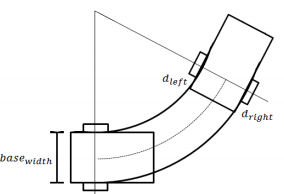
\includegraphics[width=\textwidth]{figs/dif_drive_1}
        \caption{}
        \label{fig:dif_drive_1}
    \end{subfigure}
    ~ %add desired spacing between images, e. g. ~, \quad, \qquad, \hfill etc. 
      %(or a blank line to force the subfigure onto a new line)
    \begin{subfigure}[b]{0.4\textwidth}
        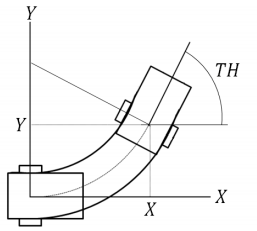
\includegraphics[width=\textwidth]{figs/dif_drive_2}
        \caption{}
        \label{fig:dif_drive_2}
    \end{subfigure}
    \caption{Modelo genérico de movimentação diferencial}\label{fig:dif_drive}
\end{figure}

O modelo descreve o deslocamento linear do robô (\emph{Dc}, equação \ref{eq:Dc}) através da média de movimentação das rodas esquerda e direita, na figura \ref{fig:dif_drive_1} identificadas como $d_{left}$ e $d_{right}$. Estes deslocamentos são obtidos através da relação entre o perímetro das rodas (R), as leituras (vulgarmente conhecidas como \emph{ticks}) de seus sensores ($ticks_{left}$ e $ticks_{right}$), os \emph{encoders}, e a quantidade de \emph{ticks} por rotação ($N_{ticks~per~rotation}$), como visto nas equações \ref{eq:dleft} e \ref{eq:dright}.  A orientação angular (\emph{th}, equação \ref{eq:th}) é obtida através da diferença entre os deslocamentos individuais das rodas, em relação à distância entre elas (figura \ref{fig:dif_drive_1}, \emph{base\textsubscript{width}}) \cite{tcc_alex}. Ou seja:

\begin{equation}
    d_{left} = \frac{2 \times \pi \times R \times ticks_{left}}{N_{ticks~per~rotation}}
    \label{eq:dleft}
\end{equation}

\begin{equation}
    d_{right} = \frac{2 \times \pi \times R \times ticks_{right}}{N_{ticks~per~rotation}}
    \label{eq:dright}
\end{equation}

\begin{equation}
    Dc = \frac{d_{left} + d_{right}}{2}
    \label{eq:Dc}
\end{equation}

\begin{equation}
    th = \frac{d_{left} - d_{right}}{base_{width}}
    \label{eq:th}
\end{equation}

Para determinar, enfim, a posição cartesiana do robô no ambiente juntamente com sua orientação angular atual (considerando estas inicialmente como $[X,Y,TH]\,\, = \,\,[0,0,0]$), utiliza-se as relações \ref{eq:cart_pos_th}, \ref{eq:cart_pos_x} e \ref{eq:cart_pos_y} definidas abaixo:

\begin{equation}
    TH = TH + th
    \label{eq:cart_pos_th}
\end{equation}

\begin{equation}
    X = X + Dc \times cos\left(\frac{th+TH}{2}\right)
    \label{eq:cart_pos_x}
\end{equation}

\begin{equation}
    Y = Y + Dc \times sen\left(\frac{th+TH}{2}\right)
    \label{eq:cart_pos_y}
\end{equation}

Essas três coordenadas representam a posição e orientação atuais do robô. Estas equações são utilizadas na implementação para aplicar a mesma movimentação realizada pelo robô às partículas. Sua implementação pode ser vista no código \ref{lst:f_estimate_p}, na seção \ref{subsec:predição}.

%\todo{Favor revisar esta seção. Coloquei o TCC do alexandre como referência número 8.}

\subsection{Predição}
\label{subsec:predição}
Como discutido anteriormente, a etapa de predição é responsável por aplicar às partículas uma movimentação teoricamente idêntica à realizada pelo robô.
Este modelo é aplicado às partículas através da função \emph{F\_estimate\_p}, que pode ser vista no Código~\ref{lst:f_estimate_p}.

%\begin{figure}[h!]
%    \centering
%    \includegraphics[scale=0.4]{figs/f_estimate_p}
%    \caption{Código que implementa o modelo de movimentação das partículas}
%    \label{fig:f_estimate_p}
%\end{figure}

%\lstinputlisting[style=customMatlab]{code/f_estimate_p.m}
\lstinputlisting[language=matlab,caption=Código que implementa o modelo de movimentação das partículas,label={lst:f_estimate_p},basicstyle=\tiny]{code/f_estimate_p.m}
% Renan, vc pode escolher o estilo do matlab, mas me parece q o default parece bom o suficiente.
% vc tb nao precisa colocar o codigo tal e qual no github. Na documentacao vc pode dar uma simplificada no codigo, remover algumas partes menos relevante, remover/alterar cometarios q tem no codigo. Isso ajudaria o relatorio nao ficar tao massante com MUUUUITO código fonte. Ou seja, não exagere no uso de código fonte. Alem disto, 'atirar' o código fonte no relatório não é o suficiente, vc deve explicá-lo.
% veja https://en.wikibooks.org/wiki/LaTeX/Source_Code_Listings para aprender a colocar codigo

Sendo objetivo principal do filtro de partículas a estimativa precisa da posição, o modelo de movimentação aplicado às partículas determina em grande parte a precisão das etapas seguintes. Porém, como não é possível construir o modelo ideal, são aplicadas variações na translação e rotação aplicadas às partículas, para compensar os distúrbios e incertezas não inclusos no modelo \cite{pftuto}. A implementação destas variações pode ser vista no algoritmo da figura \ref{fig:sample_odometry}, que descreve a função \emph{F\_sample\_odometry}, utilizada no código \ref{lst:matlab_filter_loop}, do Filtro.\par
Esta variação é descrita como um modelo RTR (\emph{Rotação, Translação, Rotação}), onde o movimento é decomposto em três passos: Uma rotação ($\delta_{rot1}$), seguido de uma translação em linha reta ($\delta_{trans}$) e então outra rotação ($\delta_{rot2}$), como pode-se ver na figura \ref{fig:rtr_model}. Evidentemente, para cada posição de partículas há um conjunto de parâmetros $[\delta_{rot1}\,\,\delta_{trans}\,\,\delta_{rot2}]^T$, sendo este considerado corrompido por distúrbios e incertezas do ambiente \cite{THR05}. Desta forma, calcula-se uma distribuição de probabilidade, que será aplicada na posição das partículas.\par

\begin{figure}[h!]
    \centering
    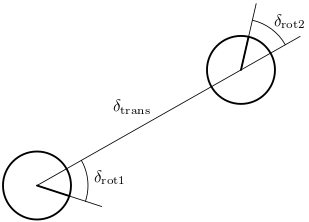
\includegraphics[scale=0.6]{figs/rtr_model}
    \caption{Modelo de movimentação RTR}
    \label{fig:rtr_model}
\end{figure}

\begin{figure}[h!]
    \centering
    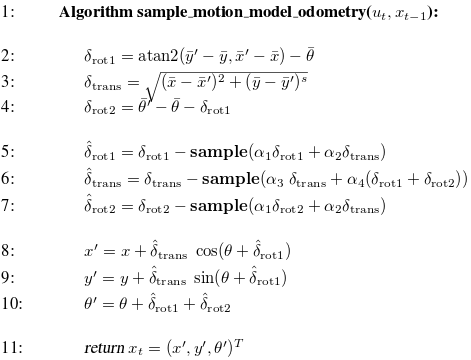
\includegraphics[scale=0.6]{figs/sample_odom}
    \caption{Algoritmo que implementa variação RTR nas partículas}
    \label{fig:sample_odometry}
\end{figure}

Olhando novamente ao algoritmo na figura \ref{fig:sample_odometry}, pode-se ver as diferentes partes deste algoritmo \cite{THR05}:

\begin{enumerate}
    \item As linhas 2 a 4 estimam o primeiro conjunto de rotações e translação que o robô teria feito.
    \item Nas linhas 5 a 7 são calculados os parâmetros de movimentação relativa, referente às poses anterior e atual. Juntamente, é inserida uma perturbação nestes parâmetros, dada por uma distribuição normal, na função \emph{sample}.
    \item Finalmente, nas linhas 8 a 10 são calculadas as probabilidades de erro para o conjunto de coordenadas $[X\,\,Y\,\,TH]$, que são somadas à posição atual, resultando assim na nova posição variada da partícula.
\end{enumerate}

Ainda na mesma figura, pode-se ver os parâmetros $[\alpha_1\,\,..\,\,\alpha_4]$. Estes são parâmetros de variação específicos do robô utilizado na simulação. Eles descrevem o efeito dos tipos de movimentações em relação a outros, ou a eles mesmos, como segue:

\begin{enumerate}
    \item \textalpha\textsubscript{1}: Efeito da rotação nas rotações.
    \item \textalpha\textsubscript{2}: Efeito da translação nas rotações.
    \item \textalpha\textsubscript{3}: Efeito da translação nas translações.
    \item \textalpha\textsubscript{4}: Efeito da rotação nas translações.
\end{enumerate}

Infelizmente, não há uma metodologia precisa para a determinação destes parâmetros. Eles devem ser otimizados empiricamente, dependendo muito de diversas variáveis (e.g. tipo de robô, parâmetros construtivos, etc), sendo esta uma das grandes resalvas do algoritmo do Filtro de Partículas. Na figura \ref{fig:odom_variation}, pode-se ver os efeitos da variação na posição. \textbf{renan, seria bom explicar estas 3 figuras abaixo o que cada uma representa.} \textbf{ficou bom assim?}

\begin{figure}[h!]
    \centering
    \begin{subfigure}[b]{0.25\textwidth}
        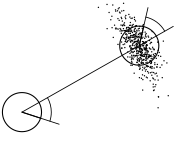
\includegraphics[width=\textwidth]{figs/odom_variation_1}
        \caption{Efeito das translações e rotações ($\alpha_2$ e $\alpha_4$)}
        \label{fig:odom_variation_1}
    \end{subfigure}
    ~ %add desired spacing between images, e. g. ~, \quad, \qquad, \hfill etc. 
      %(or a blank line to force the subfigure onto a new line)
    \begin{subfigure}[b]{0.25\textwidth}
        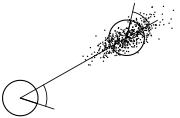
\includegraphics[width=\textwidth]{figs/odom_variation_2}
        \caption{Efeito das translações ($\alpha_3$)}
        \label{fig:odom_variation_2}
    \end{subfigure}
    ~
    \begin{subfigure}[b]{0.25\textwidth}
        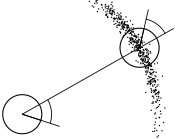
\includegraphics[width=\textwidth]{figs/odom_variation_3}
        \caption{Efeito das rotações ~~~~($\alpha_1$)}
        \label{fig:odom_variation_3}
    \end{subfigure}
    \caption{Efeito das variações na posição das partículas}
    \label{fig:odom_variation}
\end{figure}

%\todo{Favor revisar a partir da página 12, "Esta variação é descrita..."}

\subsection{Atualização}
\label{subsec:atualização}
Nesta etapa, o algoritmo atualiza o "peso"~(probabilidade) das partículas de acordo, no caso, com uma distribuição gaussiana. Para tanto, é feita uma comparação entre os dados do sensor de distância do robô e das partículas, denominado \emph{sonars}. Como trata-se de um ambiente de simulação, este sensor também é simulado, imitando um sensor de distância a laser através do algoritmo de \emph{Ray Casting}. Ray casting é uma técnica muito utilizada em computação gráfica, que calcula a distância entre dois pontos traçando um "raio" entre o ponto de origem até uma intersecção (no caso, uma parede) \cite{raycasting}. Uma limitação evidente deste, porém, é que é necessário haver um mapa conhecido do ambiente a ser navegado, sendo impossível utilizar esta técnica em ambientes dinâmicos (que mudam constantemente). O algoritmo de \emph{Ray Casting} é implementado pela função \emph{Fast\_ray\_cast}, utilizada no código do Filtro.\par

O algoritmo implementado nesta função pode ser visto na figura \ref{fig:raycast_alg}. Ele recebe como entrada a posição de uma partícula, já com a variação da etapa de predição conforme discutido previamente, e um vetor de medições de distância do robô em sí. Na primeira linha, a posição da partícula é comparada com as coordenadas do mapa. Se a partícula encontra-se fora do mapa ou em uma parede, esta recebe a probabilidade zero ($\omega\,\,=\,\,0$). Caso contrário, o algoritmo simula cada sensor (\emph{N\textsubscript{z}} sendo o número de sensores) através do \emph{Ray Casting} nas linhas 5 a 16. A variável $\Gamma_z$ corresponde a um vetor com as orientações angulares de cada sensor, em referência ao plano ordenado central do robô. A condição de parada do raio encontra-se na linha 15, que dita se o raio chegou a algum obstáculo, e na linha 11, que dita se foi alcançada a distância máxima permitida pelo sensor. Na linha 18, é feita uma comparação entre a distância calculada pelo \emph{Ray Casting} e o valor real de distância medido pelo sensor do robô \emph{z(i)}, através de uma função de distribuição gaussiana de média \emph{d} e covariância \emph{$\sigma_z$}. Finalmente, na linha 20, o algoritmo retorna uma medida de probabilidade ou peso associada a cada partícula.

\begin{figure}[h!]
    \centering
    \begin{subfigure}[b]{0.4\textwidth}
        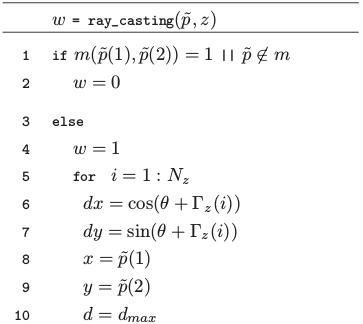
\includegraphics[width=\textwidth]{figs/raycast_alg_1}
        \caption{}
        \label{fig:raycast_alg_1}
    \end{subfigure}
    ~ %add desired spacing between images, e. g. ~, \quad, \qquad, \hfill etc. 
      %(or a blank line to force the subfigure onto a new line)
    \begin{subfigure}[b]{0.4\textwidth}
        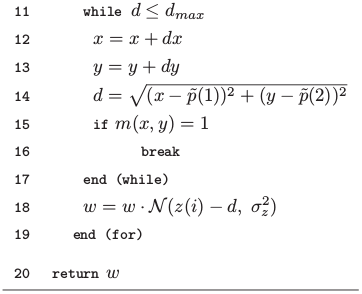
\includegraphics[width=\textwidth]{figs/raycast_alg_2}
        \caption{}
        \label{fig:raycast_alg_2}
    \end{subfigure}
    \caption{Algoritmo de \emph{Ray Casting}}
    \label{fig:raycast_alg}
\end{figure}

% renan, se vc quiser manter duas colunas de texto, tem como http://tex.stackexchange.com/questions/34098/two-column-code-listings-in-appendix-in-a-one-column-report

%begin{multicols}{2}
%\lstinputlisting[numbers=left,language=matlab,xleftmargin=3em,caption=Código que implementa o algoritmo de \emph{Ray Casting},label={lst:raycasting}]{code/raycast.m}
%\end{multicols}

A função que implementa este algoritmo é utilizada em dois trechos de código. O primeiro uso está antes do algoritmo do filtro, para calcular os dados de distâncias do robô até as paredes do ambiente onde ele circula, e o segundo uso está no código principal do filtro (\ref{lst:matlab_filter_loop}). Esta função retorna cinco medidas de distância, simulando um sensor com campo de visão de 180 graus, com medidas espaçadas em 45 graus, como demonstrado na animação da figura~\ref{fig:ambiente}.

%\begin{figure}[h!]
%    \centering
%    \includegraphics[scale=0.8]{figs/ambiente}
%    \caption{Ambiente de simulação (robô em um mapa bidimensional)}
%    \label{fig:ambiente}
%\end{figure}

% Teste de animação
\begin{figure}
    \centering
    \animategraphics[controls,loop,height=8cm]{7}{figs/animate/ambiente/ambiente-}{0}{3}
    \caption{Animação que demonstra a núvem de partículas convergindo para a localização real do modelo do robô.}
    \label{fig:ambiente}
\end{figure}

%\todo{Animate!}

\subsection{Reamostragem}
\label{subsec:reamostragem}
Um dos problemas que surge para o algoritmo do filtro de partículas é que com a variância incluida na movimentação das partículas, as partículas dispersam, e após algumas iterações elas estão tão separadas que já estão fora do mapa do ambiente ou que suas probabilidades são tão pequenas que não contribuem para a determinação da posição \cite{pftuto}. Para evitar isto, realiza-se a etapa da reamostragem, para ajustar a população de partículas baseando-se em suas probabilidades. Existem diversas formas de realizar esta etapa - eliminando as partículas com probabilidades abaixo de um certo nível e duplicando as partículas com probabilidades acima \cite{pftuto}. Por exemplo, neste trabalho foi utilizado o método da \emph{roda de reamostragem}, cuja implementação pode ser vista no código \ref{lst:sampling_wheel}.\newpage

\lstinputlisting[language=matlab,caption=Código que implementa o algoritmo da \emph{roda de reamostragem},label={lst:sampling_wheel}]{code/sampling_wheel.m}

O algoritmo da \emph{roda de reamostragem} funciona da seguinte maneira \cite{resampling}:

\begin{itemize}
    \item Primeiramente, considera-se uma roda, onde cada partícula possui uma parcela proporcional a seu peso, como pode ser visto na figura \ref{fig:samplingwheel}.
    \item Em seguida, determina-se um índice através de uma distribuição uniforme - por exemplo, determina-se um índice aleatório (no código, chamado de \emph{index}) de 1 até o número de partículas, no caso, \emph{N\textsubscript{p}}, como pode ser visto na linha 2 do código \ref{lst:sampling_wheel}.
    \item De posse do índice aleatório, é inicializada uma variável chamada \textbeta{} como zero (linha 3), obtém-se o maior peso entre as partículas (linha 4) e constrói-se o laço de repetição que percorre toda a população de partículas. Neste laço, é definido um novo valor de \textbeta, em função do valor deste somado uma distribuição aleatória de 0 até duas vezes o maior valor de peso entre as partículas (linha 6).
    \item A seguir no laço, é verificado se o peso da partícula atual não é suficiente para cobrir o valor de \textbeta{} - ou seja, se \emph{Peso atual < \textbeta}, o valor do peso é subtraido de \textbeta{} e o índice \emph{index} é incrementado em 1 (linhas 7 a 13).
    \item No caso contrário, onde \emph{$Peso \,\, atual \ge \beta$}, a partícula é selecionada (linha 14).
\end{itemize}

Desta forma, o algoritmo seleciona as partículas proporcionalmente a seu peso. Se uma partícula ocupa uma parcela maior da roda, ela será selecionada mais vezes. Não obstante, ainda é possível para este algoritmo selecionar partículas com probabilidade mediana, o que evita que o filtro de partículas torne-se tendencioso, isto é, que as partículas tendam a uma probabilidade alta, efetivamente eliminando o tão necessário efeito da variância no movimento das mesmas.

\begin{figure}[h!]
    \centering
    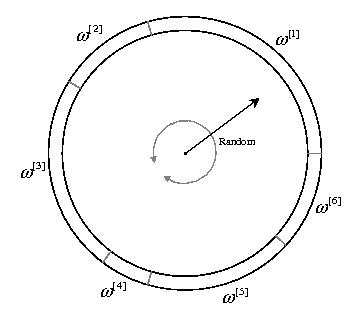
\includegraphics[scale = 0.7]{figs/samplingwheel}
    \caption{Roda de reamostragem}
    \label{fig:samplingwheel}
\end{figure}

\subsection{Outras funções}
\label{subsec:outras_funções}
Para o funcionamento do filtro, ao menos nesta implementação, são necessárias ainda outras funções que não são diretamente relacionadas ao algoritmo. Por exemplo, um pré-requisito para a utilização do filtro é que haja um mapa conhecido do ambiente onde o robô irá trafegar (métodos de navegação sem mapa são conhecidos como \emph{Simultaneous Localization And Mapping}, SLAM). Este mapa é construído no ambiente de simulação como uma matriz binária, onde o valor 1 representa uma área com parede. A função que realiza a inicialização do mapa no MATLAB pode ser vista na figura \ref{fig:loadmap}.

\begin{figure}[h!]
    \centering
    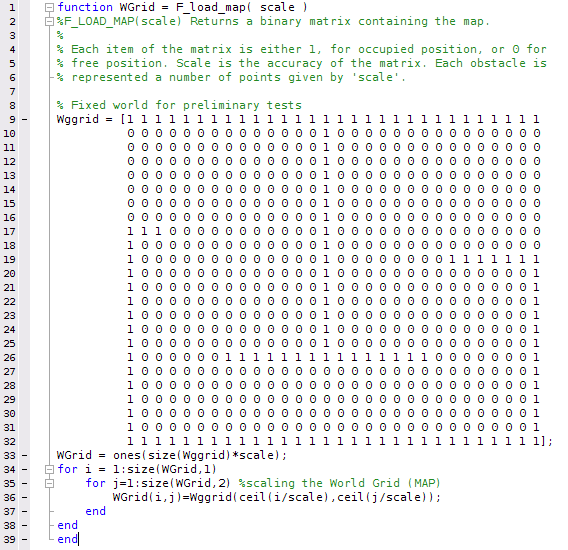
\includegraphics[scale = 0.45]{figs/loadmap}
    \caption{Função de inicialização do mapa}
    \label{fig:loadmap}
\end{figure}
\newpage

Além desta função, há as funções que realizam a simulação de movimento do robô. Uma delas é a função nativa do MATLAB, \emph{ode23}, que soluciona uma equação diferencial baseada em uma função definida pelo usuário, vista no código \ref{lst:drivecar}.

%\begin{figure}[h!]
%    \centering
%    \includegraphics[scale = 0.5]{figs/drivecar}
%    \caption{Função de simulação de movimentação do robô}
%    \label{fig:drivecar}
%\end{figure}


\begin{lstlisting}[language=matlab,numbers=left,basicstyle=\tiny, caption={Função de simulação de movimentação do robô.}, label=lst:drivecar]
function dx = F_dif_drive_car(t,x,vr,vl,R,L)
% ----------------------------------------------------------------------
%%F_dif_drive_car(t,x,vr,vl,R,L) Simulate a differential drive car
%
%   Receives the initial pose p0 = [x0 y0 th0], the velocities of the 
% wheels and the simulation time "T". Returns, the car pose p = [x y th].
% ----------------------------------------------------------------------
dx = zeros(3,1);
    dx(1) = R/2*(vr+vl)*cos(x(3));
    dx(2) = R/2*(vr+vl)*sin(x(3));    
    dx(3) = R/L*(vr-vl);
end\end{lstlisting}


%Não encontrei menção a essa função no material do Salton

%Por fim, há a função que simula os sensores de encoder nas rodas do robô, vista na figura \ref{fig:encoders}. Similarmente à função de \emph{Ray Casting}, esta função é de suma importância para o funcionamento do filtro, pois os dados calculados nesta serão utilizados na etapa de predição do filtro.

%\begin{figure}[h!]
%    \centering
%    \begin{subfigure}[b]{0.45\textwidth}
%        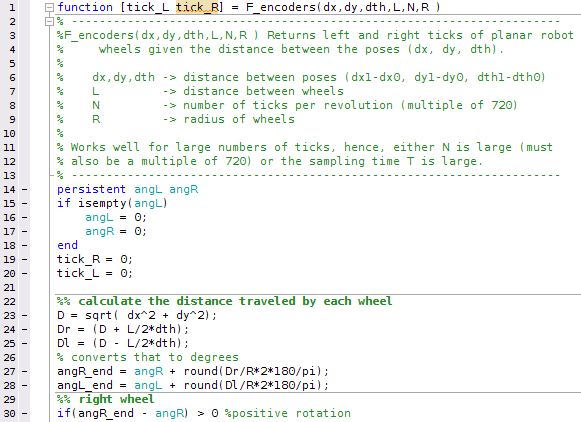
\includegraphics[width=\textwidth]{figs/encoders1}
%        \label{fig:encoders1}
%    \end{subfigure}
%    ~ %add desired spacing between images, e. g. ~, \quad, \qquad, \hfill etc. 
      %(or a blank line to force the subfigure onto a new line)
    %\begin{subfigure}[b]{0.45\textwidth}
    %    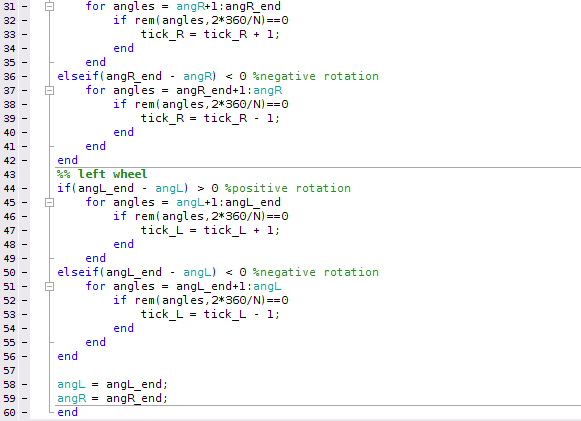
\includegraphics[width=\textwidth]{figs/encoders2}
    %    \label{fig:encoders2}
    %\end{subfigure}
    %\caption{Função de simulação de medidas dos %encoders}\label{fig:encoders}
%\end{figure}

\section{MATLAB\texttrademark + MEX}
\label{sec:matlab_mex}

Apesar dos custos computacionais elevados do MATLAB, ele traz consigo muitas vantagens para verificação e validação do algoritmo do filtro, como por exemplo a sua interface gráfica que permite a visualização do ambiente de simulação, como visto na figura \ref{fig:ambiente}. Em vista disso, decidiu-se primeiramente realizar a implementação em uma linguagem intermediária, unindo as funcionalidades do MATLAB com uma linguagem que permitisse maior desempenho nas tarefas computacionalmente mais intensivas. Assim, foi realizada a implementação no framework MEX do MATLAB. MEX (\emph{MATLAB Executable}) permite estender o Matlab criando funções em C/C++ e acessá-las como se estas funções fossem próprias do Matlab. Outra vantagem é que a função desenvolvida em MEX é compilada ao invés de interpretada como o MATLAB, trazendo ganhos de desempenho.

%é uma extensão - é extremamente popular com desenvolvedores de aplicações paralelas, por possibilitar programação em linguagens C e C++ com suporte a paradigmas de programação como CUDA, por exemplo. Efetivamente, um arquivo MEX é um programa escrito em linguagem C ou C++, que é compilado pelo MATLAB e executado em um script normal como uma função \cite{mex}. 

Para utilização do MEX, existe uma estrutura pré-definida para qualquer programa. Esta consiste em uma função principal, chamada de função de entrada (\emph{mexFunction}), onde são definidas as variáveis utilizadas no procedimento que se deseja implementar, além das variáveis de saída, que serão repassadas ao programa do MATLAB, visto que os ambientes de execução do MATLAB e das funções MEX são distintos. Nesta função também é chamada a rotina principal que deseja-se executar, que também é definida no mesmo arquivo MEX. Esta leva como parâmetros as variáveis de entrada (que recebem os valores passados na chamada de função no MATLAB), e as variáveis de saída.

Neste trabalho foi implementado inteiramente o laço principal do filtro, juntamente com as funções auxiliares necessárias ao laço em um único arquivo MEX, que encontra-se disponível no arquivo \emph{mexFP.c}, diretório \emph{src/matlab\_mex} do repositório do projeto no GitHub. O uso de MEX causou um grande ganho de desempenho, o que será discutido no Capítulo~\ref{sec:results}.

\section{Linguagem C}
\label{sec:linguagem_c}

%\todo{A completar, JANEEE}

Esta implementação do programa, disponível no diretório \emph{src/c}, é um passo adicional no sentido em desvincular o filtro do ambiente MATLAB. A versão MATLAB + MEX executa o programa no ambiente do MATLAB, mas com a maior parte do filtro implementada em C. A versão apresentada nesta seção executa o filtro totalmente fora do ambiente MATLAB. Entretando, para compilar este programa ainda é necessário ter o MATLAB instalado pois ele utiliza a biblioteca \emph{mat.h} que permite ler arquivos \emph{.mat}.

Estes arquivos \emph{.mat} são usados para ler os inputs do filtro, como dados de odometria do carro, mapa, sonares, entre outros parâmetros. Esta leitura é realizada nas funções setDynamicVariables(), setStaticVariables(), setCarPosition().
Ao final do programa outro arquivo \emph{.mat} é gerado com a posição das partículas calculadas pelo filtro ao longo do tempo. Este arquivo é então carregado no MATLAB simplesmente para fins de visualização dos resultados em formato gráfico, usando o rescurso de animação da versão original do filtro.

A parte principal do código está representada no código~\ref{lst:c-filter}.

\begin{lstlisting}[style=customc,numbers=left,caption={Parte principal da implementação em C do filtro.}, label=lst:c-filter]
ode23(k);   // estimate the actual car position

fastRayCasting(x[k+1],y[k+1],th[k+1], 1, k, temp);  // estimate the sonar position

F_encoders(x[k+1]-x[k],y[k+1]-y[k],th[k+1]-th[k], k); // encoders
double odo[3] = {x[k], y[k], th[k]};
F_estimate_p(odo, k); 

particleFilter(k);  // execute the k iteration of the filter

memcpy((void *)(mxGetPr(p_temp)), (void *)p, p_M*p_N*sizeof(p)); // save particle position into .mat
\end{lstlisting}


\subsection{Otimização na representação do mapa}
Uma das otimizações realizadas nesta versão do filtro foi na representação do mapa do ambiente simulado. Em MATLAB o mapa é representado por uma matriz onde cada campo da matriz representa um tipo de dados de tipo \emph{float}, que ocupa 8 bytes em memória. Sendo uma matriz binária, isto representa uma desperdício de memória significativo, especialmente para mapas grandes. A solução adotada foi codificar o mapa em uma matriz onde cada posição do mapa ocupasse somente um bit em memória. Isto siginifica que cada byte de memória representa 8 posições do mapa. Em relação ao mapa em MATLAB, isto representa uma redução de 64 vezes de uso de memória para o mapa.

O ganho desta nova representação não se resumo somente em redução de uso de memória. Como os computadores possuem hierarquia de memória e memórias cache, isto significa que com uma representação mais compacta do mapa, a quantidade de \emph{cache miss} vai reduzir drasticamente, aumentando o desempenho geral do programa.

Foi desenvolvida uma função de conversão da representação original do mapa em MATLAB chamada de \emph{resize\_map}. Ela recebe como entrada um ponteiro para o mapa desotimizado (map), para o mapa otimizado (map\_opt), e as dimensões do mapa (row e col). 

\begin{lstlisting}[style=customc,numbers=none]
int resize_map(double *map, char *map_opt, int row, int col)
\end{lstlisting}

Como a linguagem C não acessa diretamente tipo bit de dados, foi desenvolvida uma macro auxiliar que converte a forma original de acessar o mapa (assumindo \emph{row} linhas e \emph{col} colunas), mas usando a nova representação compacta do mapa. O trecho do código da macro GETPIXEL(i,j) está apresentado abaixo. Basicamente ela converte i e j para acessar o bit correto da matriz que representa o mapa. O retorno é '1' se a posição está ocupada ou '0' caso contrário.

\begin{lstlisting}[style=customc,numbers=none,basicstyle=\footnotesize]
#define GETPIXEL(i,j) (((map_opt[i*col_opt+(j/8)] & (1<<(7-(j%8)))) != 0) ? 1:0)
\end{lstlisting}

Futuramente, ao invés de ler o mapa em MATLAB, este programa pode ler uma mapa em bitmap binário codificado para representar 1 pixel por bit. Isto simplificaria a descrição de mapas diferentes pois bastaria editar o novo mapa em um software tipo GIMP. Pensando nisto foi desenvolvido um programa chamado \emph{bmp2hex}, disponível no diretório \emph{test}, que converte o arquivo bmp para um formato compacto e mais simplificado. Alternativamente o filtro também poderia ler diretamente o bitmap, sem passar pela conversão realizada pelo programa \emph{bmp2hex}.


\section{Simulador STAGE}
\label{sec:stage}

Ainda pensando em uma forma de facilitar a visualização e validação de resultados, optou-se por investigar a implementação do algoritmo do filtro no simulador robótico STAGE \cite{vaughan2008massively}, que já é consolidado no ramo da robótica. Ele funciona utilizando um formato de arquivos específico, sendo o arquivo principal o "mundo". Este arquivo define o mapa, chamado \emph{floorplan}, os atores (robôs) e os arquivos que irão ditar o comportamento dos atores. O \emph{floorplan}, por sua vez, é definido por uma imagem em escala de cinza, o que é extremamente interessante pois permite facilmente a mudança de ambientes de navegação, sem a necessidade da tarefa trabalhosa de montar manualmente uma matriz binária como acontecia no MATLAB. Um exemplo do ambiente de navegação do MATLAB  (figura \ref{fig:ambiente}), reproduzido no STAGE, pode ser visto na animação da figura~\ref{fig:stage-anim}.

\begin{figure}
    \centering
    \animategraphics[controls,loop,height=8cm]{7}{figs/animate/stage/stage_anim-}{1}{4}
    \caption{Animação do ambiente de simulação reproduzido no STAGE}
    \label{fig:stage-anim}
\end{figure}

Os outros arquivos, que ditam o comportamento dos atores no mundo, são escritos na linguagem C++. Nestes arquivos, foram implementados o algoritmo do filtro e o comportamento de movimentação do robô no ambiente de navegação. Uma versão resumida do código principal de implementação do filtro, que encontra-se no arquivo que dita o comportamento do robô, pode ser visto no código \ref{lst:random_particles_redux}.

\lstinputlisting[language=c++,caption=Código resumido do algoritmo do Filtro de Partículas no STAGE,label={lst:random_particles_redux},basicstyle=\tiny]{code/random_particles_redux.cc}

Neste código, pode-se ver claramente as etapas do filtro, sendo a etapa de predição realizadas nas linhas 6 a 13, a etapa de atualização nas linhas 15 a 39 e a etapa de reamostragem nas linhas 48 a 80. As etapas foram fielmente transcritas tal como elas são na implementação em MATLAB, com algumas peculiaridades que são exclusivas ao STAGE, como a linha 4 por exemplo, que recupera o modelo da partícula do mundo simulado pelo STAGE. Esta partícula tem diversas propriedades, sendo a mais interessante a sua pose (posição 2d + orientação angular), que é recuperada na linha 8. Uma grande facilidade deste simulador é que não é preciso modelar os sensores, sendo que o próprio STAGE já nos proporciona os dados dos robôs e sensores simulados. O código completo pode ser encontrado no repositório do projeto, no arquivo \emph{random\_particles.cc} da pasta \emph{/stage/examples/ctrl}.\par

O arquivo de mundo, por sua vez, determina os parâmetros do ambiente de simulação, como qual imagem (em escala de cinza) será utilizada para construir o ambiente, os atores que popularão o mundo (e.g. pessoas, robôs), suas geometrias e comportamentos, entre outros. O código \ref{lst:random_world_redux} apresenta, também de forma reduzida, o arquivo de mundo utilizado com a implementação do filtro. O código completo, novamente, encontra-se no repositório do projeto, na pasta \emph{/stage/worlds} sob o nome de \emph{random\_particles.world}.

\lstinputlisting[caption=Arquivo de mundo resumido,label={lst:random_world_redux},basicstyle=\tiny]{code/random_world_redux.world}

As linhas 3 a 10, no código \ref{lst:random_world_redux}, realizam a parmetrização do \emph{floorplan}, que é o ambiente onde irá trafegar o robô. Escolhe-se nome, tamanho, orientação e a imagem no qual o ambiente será baseado. A seguir, nas linhas 13 a 28, define-se o robô, ditando seu nome, pose inicial, comportamento (linha 23) e qual o tipo de modelo de movimentação ele utilizará (linha 26). Este no caso é odometria, por ser um modelo ruidoso no STAGE, sendo similar ao modelo em MATLAB e à vida real. Na linha 20, porém, há a descrição do sensor de distância, aqui descrito como uma generalização do sensor de distância a laser SICK\footnote{\url{https://www.sick.com/de/en/detection-and-ranging-solutions/2d-laser-scanners/tim3xx/c/g205751}}. A seguir, tem-se a definição do modelo base de onde serão criadas as partículas, nas linhas 31 a 42. Sua geometria é definida na função \emph{puck}, nas linhas 45 a 60, que entre outros define os parâmetros de execução do mundo em sí (número de partículas, nome do robô e floorplan a ser carregado), na linha 59.\par

Porém, a curva de aprendizado do STAGE pode vir a ser um tanto elevada. Por sorte, há diversos exemplos de simples aplicações e instruções de uso no repositório do simulador\footnote{\url{https://github.com/rtv/Stage}}. É incluído como anexo neste relatório um passo-a-passo de compilação e instalação do STAGE.

%\todo{Apresentar código random\_particles resumido com explicações das três etapas do filtro}
%\todo{Botar exemplo de arquivo de mundo e explicar}
%\todo{Botar passo-a-passo como anexo sobre como baixar e compliar o stage}

%\todo{acho q vc deve incluir um esqueleto resumido do codigo do stage. pelo menos descrevendo brevemente os trechos principais, a principais funcoes usadas, as principais estruturas de dado, como parametrizar a execucao, como compilar o codigo, ....}

%---------------------------------------------------------
% Resultados
% ----------------------------------------------------------
\chapter[Resultados]{Resultados}
\label{sec:results}

\section{Estudos iniciais}
\label{sec:estudos_iniciais}
Inicialmente, foi realizado um estudo detalhado da implementação original do professor Salton, para que fosse possível entender seu funcionamento e assim determinar quais eram os pontos críticos em tempo computacional da implementação. Em outras palavras, era de interesse descobrir quais funções ocupavam uma maior porcentagem do tempo de execução total. Para tanto, foi utilizada a ferramenta de \emph{profiling} do próprio MATLAB, que mede o tempo de execução total e individual de cada função. Na figura \ref{fig:matlab_profile} pode-se ver um exemplo de execução do código com esta ferramenta, de forma reduzida. Analisando os tempos, encontrou-se que o ponto crítico da implementação é a função de \emph{Ray Casting}, que ocupa 42,99 segundos dos 51,63 segundos de execução total do algoritmo (83,26 \%). Logo em seguida segue a função \emph{ode23}, que é responsável pela simulação do robô diferencial, ocupando 4,12 \% do tempo de execução. Os 12,62 \% restantes são compostos de todas as outras funções utilizadas, algumas referentes à implementação em sí (e.g. \emph{F\_measurProb}, \emph{F\_sample\_odometry}) e outras referentes a funções internas do MATLAB (e.g. \emph{imshow}, \emph{movegui}).

\begin{figure}[h!]
    \centering
    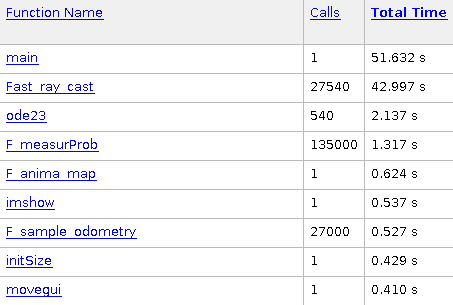
\includegraphics[scale=0.7]{figs/matlab_profile}
    \caption{Tempos de execução do código em MATLAB}
    \label{fig:matlab_profile}
\end{figure}

Assim, fica evidente que a otimização toma prioridade no algoritmo de \emph{Ray Casting}. Após estudos e experimentações deste algoritmo com diferentes parâmetros de Filtro, descobriu-se que as duas variáveis mais influentes em seu tempo computacional são o número de partículas do Filtro e o número de sensores que o \emph{Ray Casting} precisa simular para cada partícula. Desta forma, é possível estabelecer uma métrica de carga computacional $Q$, cuja unidade é a quantidade de vezes que o algoritmo de \emph{Ray Casting} precisará ser executado. 
Definindo-se que o número de partículas é $N$ e o número de sensores, que neste caso é constante, é $M\,=\,5$, tem-se a relação $Q\,=\,N\times{}M\,=\,5\times{}N$. Evidentemente, as variáveis $N$ e $M$ possuem fatores de impacto diferentes. 
Tomando como exemplo os resultados da figura \ref{fig:matlab_profile}, que foram obtidos com $N\,=\,50$, tem-se que o número de execuções fica em $Q\,=\,5\times50\,=\,250$ execuções para apenas uma iteração do Filtro. Se $N$ aumentar em 5 unidades, tem-se $Q\,=\,5\times(50\,+\,5)\,=\,275$ execuções. 
Porém, se o parâmetro $M$ aumenta em 5 unidades, tem-se $Q\,=\,(5\,+\,5)\times50\,=\,500$ execuções, que é quase o dobro. Isso torna-se evidente quando percebe-se que os sensores tem de ser simulados para cada partícula individualmente. Desta forma, conclui-se que este parâmetro é o mais crítico deste algoritmo.\par
Vale lembrar que o parâmetro $Q$ e o número de chamadas (\emph{Calls}) mostrado na figura \ref{fig:matlab_profile} são diferentes, sendo o parâmetro $Q$ representativo do número de execuções do algoritmo que encontra-se implementado na função \emph{Fast\_ray\_cast}, enquanto que o número de chamadas corresponde à quantidade de vezes que a função em sua totalidade foi chamada. É possível chegar no número de chamadas da seguinte maneira, sendo o número de iterações $k\,=\,540$ e considerando a execução do \emph{Ray Casting} para o robô, uma vez por iteração: $Calls\,=\,k\times{}N\,+\,k\,=\,540\times{}50\,+\,540\,=\,27540$ chamadas.

\section{Ganhos de desempenho}
\label{sec:ganhos_desempenho}

A seguir, foram discutidas maneiras de reduzir a carga computacional do algoritmo do Filtro. Uma solução óbvia é reduzir o parâmetro cujo impacto é maior na carga computacional, no caso o número de sensores $M$. Porém, o algoritmo já conta com um número baixo de sensores, sendo que a redução deste parâmetro comprometeria a precisão do Filtro. Outra alternativa é a redução do número de partículas $N$, que porém já estão em número bem reduzido.\par

É possível também substituir o algoritmo pelo qual os sensores são simulados, ou seja, trocando o \emph{Ray Casting} por outro método de atualização, onde foram encontrados bons resultados utilizando a técnica dos campos de probabilidade (\emph{likelihood field model}, \cite{THR05}), implementada pelo professor Salton.
Porém, posteriormente à implementação de outras técnicas de atualização, resolveu-se explorar uma outra maneira possível para redução da carga computacional: Reduzir o tempo de execução das funções em sí.\par

Desta forma, concluiu-se que era necessário uma mudança de ambiente de implementação. Como já discutido na seção \ref{sec:matlab_mex}, o MEX foi um passo intermediário para a implementação do código na linguagem C pura que por si só já mostrou uma grande redução em carga computacional, mesmo sendo o código do Filtro fielmente transposto a MEX. Na figura \ref{fig:mex_profile} pode-se ver que o tempo de execução do Filtro em sua totalidade (incluindo o algoritmo de \emph{Ray Casting}), na função \emph{mexFP}, é muito menor do que a execução somente da função de \emph{Ray Casting} na implementação original, e ocupando somente 2,97 \% do tempo de execução total do código. Comparando os tempos de execução das funções \emph{Fast\_ray\_cast} na implementação original e \emph{mexFP} na implementação MEX, tem-se que a segunda função é aproximadamente 208 vezes mais rápida. Pode-se, enfim, comparar as duas implementações com diferentes valores para o número de partículas, que é vista na figura \ref{fig:matlab_vs_mex}.

\begin{figure}[h!]
    \centering
    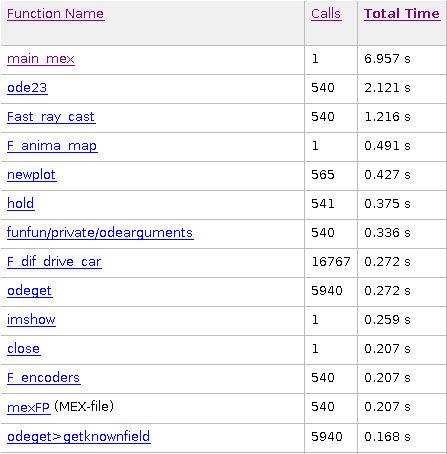
\includegraphics[scale=0.5]{figs/mex_profile}
    \caption{Tempos de execução do código com o Filtro em MEX}
    \label{fig:mex_profile}
\end{figure}

\begin{figure}[h!]
    \centering
    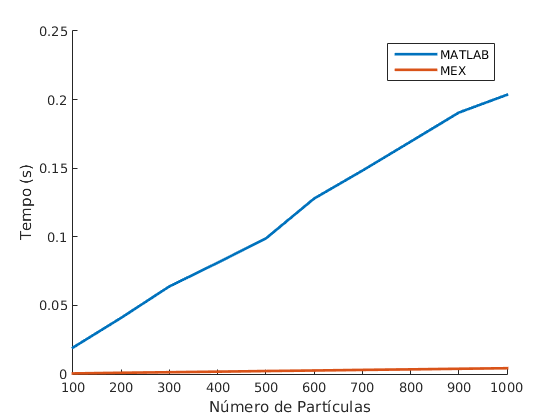
\includegraphics[scale=0.7]{figs/matlab_vs_mex}
    \caption{Gráfico comparativo dos tempos de execução do código do Filtro entre MATLAB e MEX}
    \label{fig:matlab_vs_mex}
\end{figure}

A respeito da implementação no simulador STAGE, notou-se um desempenho substancialmente inferior em relação ao MEX. Utilizando contadores de tempo no código principal do comportamento do robô no STAGE (código \textbf{XX}), pode-se ver que o Filtro nesta implementação possui tempos de execução de em média entre 0,012 e 0,014 segundos, o que é aproximadamente 5 vezes maior que os 0,0022 segundos médios de execução do Filtro em MEX. A figura \ref{fig:mex_vs_stage} mostra um gráfico comparativo entre os tempos de execução do MEX e STAGE.

\begin{figure}[h!]
    \centering
    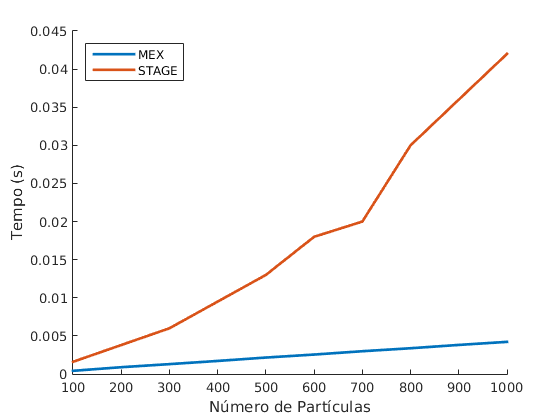
\includegraphics[scale=0.7]{figs/mex_vs_stage}
    \caption{Gráfico comparativo dos tempos de execução do código do Filtro entre MEX e STAGE}
    \label{fig:mex_vs_stage}
\end{figure}


\section{Comparação de desempenho com o AMCL}
\label{sec:amcl}

O \emph{AMCL}\footnote{\url{http://wiki.ros.org/amcl}} é o módulo do framework ROS \cite{ros-book} que executa o algoritmo de filtro de partículas. O AMCL representa o estado da arte em termos da implementação do algoritmo e, portanto, é utilizado para fins de comparação a implementação desenvolvida neste projeto.\par

Assim, decidiu-se comparar o desempenho da implementação em STAGE com este módulo. Para uma melhor comparação, foi utilizado o pacote do ROS chamado \emph{navigation\_stage}\footnote{\url{http://wiki.ros.org/navigation_stage}}, que implementa o algoritmo do AMCL utilizando algumas funções existentes no STAGE (e.g. \emph{Raytrace}). Este pacote também implementa o módulo de controle robótico \emph{move\_base} e o ambiente de simulação \emph{RVIZ}, sendo que assim fica delegado ao STAGE somente a simulação dos sensores. Na figura \ref{fig:rviz_environ}, pode-se ver o mapa de um ambiente simulado, no \emph{RVIZ}, onde a nuvem de pontos vermelhos representa a nuvem de partículas.\par

\begin{figure}[h!]
    \centering
    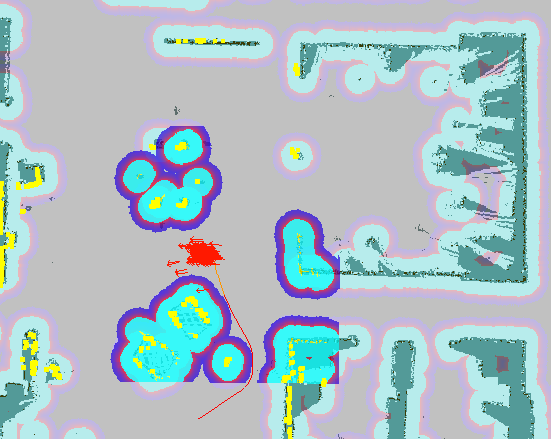
\includegraphics[scale=0.4]{figs/rviz_environ}
    \caption{Ambiente de simulação RVIZ}
    \label{fig:rviz_environ}
\end{figure}

A ferramenta de análise de utilização de processamento \emph{sysprof}\footnote{\url{http://sysprof.com/}} foi utilizada, por ter algumas vantagens em relação a outras aplicações semelhantes. Por exemplo, outra ferramenta popular é o framework \emph{Valgrind}\footnote{\url{http://valgrind.org/}}, sendo possível rodar o nodo AMCL diretamente com este profiler. A sua desvantagem frente ao \emph{sysprof}, porém, é que o nodo desta forma é executado em um ambiente virtual, utilizando uma única \emph{thread}, o que pode vir a mascarar o desempenho real do AMCL se este utilizar várias \emph{threads}. O \emph{sysprof} analisa todas as funções ativas no sistema em dado momento, assim contornando este problema. Ambas as implementações foram executadas utilizando parâmetros equivalentes, com 1000 partículas. Vale lembrar, porém, que os dados de tempos obtidos com o \emph{sysprof} não são constantes, visto que dependem do que o processador pode alocar no momento do profiling para cada função. Ele é utilizado apenas para ter uma base do desempenho das implementações AMCL e STAGE.\par

Na figura \ref{fig:sysprof_overview_stage} pode-se ver, primeiramente, um apanhado geral das funções e suas porcentagens de utilização com a implementação STAGE rodando. A figura mostra a função \emph{[stage]} ocupando 38,7 \% do tempo de utilização do processador, que é uma porcentagem bem alta. Também é possível ver as funções do STAGE \emph{ModelRanger}, mais detalhada na figura \ref{fig:sysprof_stage}, e \emph{Raytrace}. Como percebe-se pelas figuras, a função de \emph{Raytrace} aparece duplamente, uma vez fora e uma vez dentro da função \emph{ModelRanger}. Há ainda uma diferença gritante de utilização entre elas, 11 e 0,06 \% respectivamente, que se dá porque a função \emph{Raytrace} dentro da \emph{ModelRanger} é responsável pela simulação dos sensores de distância do robô, enquanto que a outra é responsável pela simulação dos sensores de distância das partículas.\par

\begin{figure}[h!]
    \centering
    \begin{subfigure}[b]{0.48\textwidth}
        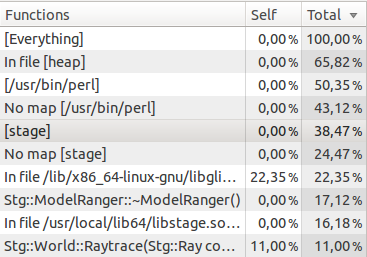
\includegraphics[width=\textwidth]{figs/sysprof_overview_stage}
        \caption{}
        \label{fig:sysprof_overview_stage}
    \end{subfigure}
    ~ %add desired spacing between images, e. g. ~, \quad, \qquad, \hfill etc. 
      %(or a blank line to force the subfigure onto a new line)
    \begin{subfigure}[b]{0.48\textwidth}
        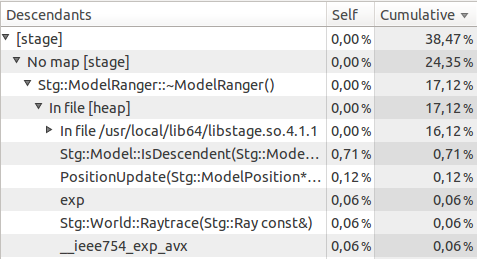
\includegraphics[width=\textwidth]{figs/sysprof_stage}
        \caption{}
        \label{fig:sysprof_stage}
    \end{subfigure}
    \caption{Profiling da implementação STAGE}
    \label{fig:sysprof_impl_stage}
\end{figure}

Já para a implementação em ROS, dada a natureza do framework de separar suas execuções em várias funções, considerou-se impraticável compor uma figura tal como a \ref{fig:sysprof_overview_stage}. Ainda assim, foram encontradas as funções relevantes ao nodo AMCL, como se por ver na figura \ref{fig:sysprof_amcl}. Nesta figura, tem-se evidência da técnica dos campos de probabilidade, utilizada na etapa de atualização, que é mais eficiente do que a técnica de \emph{Raytrace} utilizada na implementação STAGE. Também encontrou-se a função \emph{ModelRanger}, que realiza a simulação dos sensores de distância do robô (figura \ref{fig:sysprof_ranger_amcl}). Finalmente, com relação às porcentagens de utilização, percebe-se que o AMCL é de fato melhor, com uma utilização de apenas 1,35 \% em sua totalidade. A função \emph{Raytrace} aqui também possui um desempenho melhor, utilizando apenas 1,57 \% do processamento.

\begin{figure}[h!]
    \centering
    \begin{subfigure}[b]{0.6\linewidth}
        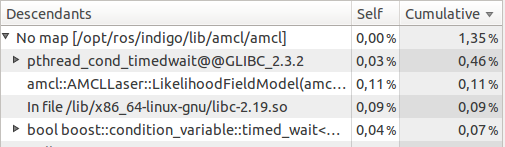
\includegraphics[width=\linewidth]{figs/sysprof_amcl}
        \caption{}
        \label{fig:sysprof_amcl}
    \end{subfigure}
    ~ %add desired spacing between images, e. g. ~, \quad, \qquad, \hfill etc. 
      %(or a blank line to force the subfigure onto a new line)
    \begin{subfigure}[b]{0.6\linewidth}
        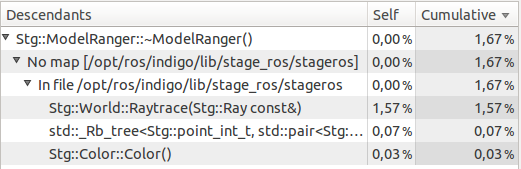
\includegraphics[width=\linewidth]{figs/sysprof_ranger_amcl}
        \caption{}
        \label{fig:sysprof_ranger_amcl}
    \end{subfigure}
    \caption{Profiling do AMCL com o pacote \emph{navigation\_stage} do ROS}
    \label{fig:sysprof_impl_amcl}
\end{figure}


% ----------------------------------------------------------
% Conclusões
% ----------------------------------------------------------
\chapter[Conclusões]{Conclusões}

Este projeto apresentou o desenvolvimento e os resultados obtidos no sentido de otimizar a execução do algoritmo de filtro de partículas. Três novas versões do filtro foram desenvolvidas, cada uma com suas vantagens e desvantagens. A versão MATLAB+MEX é muito similar à versão original, porém possui um desempenho muito melhor. Entretanto ele ainda está atrelado ao MATLAB, o que pode limitar o seu uso. A versão C executa fora do ambiente do MATLAB, mas ainda precisa que o MATLAB esteja instalado no computador para fins de visualização dos resultados obtidos. Apesar do seu desempenho não ter sido avaliado, espera-se que seja ainda melhor que a versão MATLAB-MEX. Por fim, as versão STAGE está totalmente desvinculada do MATLAB, é baseada somente em código aberto, e possui uma versatilidade muito melhor que o ambiente de simulação original baseado em MATLAB, embora seu desempenho seja menor do que a implementação em MEX. Foi também realizada uma comparação de utilização de processamento entre a implementação em STAGE e o nodo AMCL do framework ROS, que é considerada uma implementação estado da arte. Novamente, a implementação em STAGE provou-se menos eficiente, ocupando porcentagens substancialmente maiores em relação ao AMCL. Possivelmente isto seja porque o AMCL utiliza a técnica de campos de probabilidade para a etapa de atualização do Filtro, o que reduz bastante o tempo computacional desta etapa, ou também porque o algoritmo de \emph{Raytrace} seja implementado de uma maneira otimizada. As seções a seguir discutem caminhos para a continuação deste projeto.

% ----------------------------------------------------------
% Discussões
% ----------------------------------------------------------
\section{Discussões}

\subsection{Sobre a execução do algoritmo em FPGAs}

O projeto original mencionava a possibilidade de explorar o potencial paralelismo do filtro de partículas utilizando FPGAs \footnote{ Field-programmable gate array \url{https://en.wikipedia.org/wiki/Field-programmable_gate_array}}. Entretanto, ao estudar melhor o algoritmo, percebeu-se que o mesmo utiliza intensivamente de operações de ponto flutuante e operações transcendentais. A implementação destas operações em FPGA ocuparia uma grande área de lógica reconfigurável, limitando o número de operações que o FPGA suportaria em paralelo, por fim, limitando o potencial de paralelismo do algoritmo. Outra desvantagem desta abordagem é que o projeto da lógica do filtro em VHDL seria complexa, exigindo grande esforço em codificação VHDL e verificação da lógica. Estimamos que o esforço necessário seria maior que o possível considerando o número de alunos disponíveis no projeto e o tempo disposto para tal desenvolvimento. Desta forma, a opção de projetar parte do filtro em FPGA foi descartada logo no início do projeto.

\subsection{Sobre a execução do algoritmo em GPUs}

Originalmente no projeto submetido havíamos pensado em ganhar desempenho explorando o possível paralelismo do filtro, uma vez que ele repete as mesmas operações para cada partícula. Intuitivamente isto parecia factível, porém, ao estudar o algoritmo mais detalhadamente percebeu-se alguns complicações para a sua implementação em arquiteturas paralelas. 

Primeiro, a maioria das operações são em ponto flutuante. Por outro lado as GPUs atuais possuem número limitado de unidades de ponto flutuante, reduzindo o potencial de paralelismo. Por exemplo, a GPU NVIDIA Quadro 4000\footnote{\url{http://www.nvidia.com/object/product-quadro-4000-us.html}} disponível no laboratório suporta somente $4,86\times10^{11}$ operações de ponto flutuante em paralelo (single-precision). No segundo semestre de 2015 recebemos uma outra GPU com mais recursos, modelo NVIDIA Tesla K40\footnote{\url{https://www.nvidia.com/content/tesla/pdf/nvidia-tesla-k40-2014mar-lr.pdf}}. Esta GPU suporta $4,29\times10^{12}$ operações de ponto flutuante em paralelo (também single-precision), entretanto o seu custo está estimado em US\$ 3,115.42\footnote{\url{http://www.amazon.com/NVIDIA-Tesla-Graphic-Card-900-22081-2250-000/dp/B00KDRRTB8}}, limitando a utilização da versão otimizada do filtro. 

Segundo, as GPUs possuem quantidade de memória interna limitada. Quando este limite é ultrapassado, a GPU começa a utilizar a memória externa, que é muito mais lenta e possui o gargalo de largura de banda da interface externa da GPU. O principal problema do filtro é que o cálculo de cada partícula efetua leituras no mapa, que pode ocupar uma grande quantidade de memória. No caso de cálculo das partículas em paralelo, isto significa que haveriam várias leituras simultâneas para a memória que representa o mapa.  Geralmente a quantidade de memória utilizada pelo mapa ultrapassa a quantidade de memória interna da GPU, fazendo com que a mesma acesse a memória externa que é lenta e com acesso congestionado devida à limitação da largura de banda da interface.

Algumas alternativas para este segundo problema foram pensadas, porém não houve tempo de testá-las, ficando a ideia para trabalhos futuros. Como mencionado anterioremente, foi desenvolvida uma representação compacta do mapa, que ocupa 64 vezes menos memória que a representação original. Isto ajudaria a aliviar o problema, entretanto, à medida que o mapa cresça, eventualmente ele ainda não vai caber na memória interna da GPU, causando perda de desempenho. Outra alternativa promissora é o uso das memórias de constantes e de texturas \footnote{Texture Memory in CUDA | What is Texture Memory in CUDA programming \url{http://cuda-programming.blogspot.com.br/2013/02/texture-memory-in-cuda-what-is-texture.html}} existentes nas GPUs CUDA. Estas memórias possuem hierarquia de memória e são usadas em modo somente de leitura. Estas memórias são adequadas pois o mapa é somente lido duranto do cálculo das partículas.

Outra alternativa para o segundo problema, relacionado ao mapa do ambiente, seria mudar o algoritmo do programa para ele não acessar o mapa inteiro, mas sim seções do mapa. Isto permitiria colocar somente um pedaço do mapa na memória e calcular somente as partículas que estão próximas da área representada pelo mapa. Esta alternativa tem o melhor potencial de ganhos de desempenho, porém é mais complexa e exigiria mais estudos de formas alternativas de representações de mapas em memória.

%The cuda SDK contains a straightforward example simpleTexture which demonstrates performing a trivial 2D coordinate transformation using a texture.
%http://stackoverflow.com/questions/8767059/texture-memory-in-cuda-concept-and-simple-example-to-demonstrate-performance
%http://docs.nvidia.com/cuda/cuda-samples/#simple-texture

% ----------------------------------------------------------
% Trabalhos futuros
% ----------------------------------------------------------
\section{Trabalhos Futuros}

%\todo{Mencionar o artigo a ser feito, relacionar com seção discussões}

\subsection{Representar o mapa em memórias read-only da GPU}

Como mencionado antes, o uso das memórias de constantes e de texturas pode ser uma solução para colocar o mapa do ambiente nas memórias internas da GPU, potencialmente levando a um grande aumento de desempenho.

\subsection{Representações mais eficientes do mapa em memórias}

Apesar das otimizações obtidas com a representação do mapa, acreditamos que será necessário otimizar ainda mais a utilização de memória. Será necessário fazer uma revisão das possíveis representações. Por exemplo, a memória do mapa possui uma característica esparsa, onde poucas posições da memória são utilizadas, havendo desperdícios. Pode-se tentar tirar proveito desta característica para tornar a representação ainda mais eficiente e compacta. Outra possibilidade é fazer a carga em memória de seções do mapa, ao invés do mapa completo.

\subsection{Artigo sobre uso do STAGE para fins educacionais}

O uso de Stage como ferramenta de simulação do filtro mostrou-se muito promissora e versátil, permitindo facilmente mudar o ambiente simulado, suportando múltiplos robôs, possibilitando modelar facilmente os recursos típicos de um robô. Além disso o seu desempenho foi satisfatório, um pouco mais lento que a versão do filtro sozinho, sem recursos de simulação. Considerando estas vantagens, planejamos no primeiro semestre de 2016 escrever um artigo sobre o uso da implementação do filtro com STAGE para fins educacionais, explicando o funcionamento do mesmo e como as varíaveis do filtro influenciam o seu comportamento.


\subsection{Continuar a implementaçaão da versão C}

A versão C do filtro ainda tem uma dependência com o MATLAB. No futuro esta dependência pode ser eliminada e criado um pacote para facilitar a distribuição aberta do software.

\subsection{Estudar o método de Likehood Field}

O estudo do AMCL mostrou que ele utiliza um método alternativo ao Raytrace, chamado Likehood Field, que é computacionalmente mais eficiente. Seria interessante estudar mais este método para integrá-lo à implementação proposta do filtro. O uso deste método possivelmente faria com que o desempenho da implementação proposta ficasse similar ao desempenho do AMCL.

\subsection{Integrar a versão otimizada do filtro ao ROS}

Estima-se que o versão desenvolvida do filtro tenha desempenho similar ao AMCL, hoje disponível no ROS. Porém, com algumas otimizações que poderiam ser realizadas, espera-se que a nova versão seja mais rápida que o AMCL. Se isto se confirmar, seria interessante montar um novo pacote para o ROS, que substitua o AMCL atual. 

% ---
% Finaliza a parte no bookmark do PDF, para que se inicie o bookmark na raiz
% ---
\bookmarksetup{startatroot}% 
% ---

% ----------------------------------------------------------
% ELEMENTOS PÓS-TEXTUAIS
% ----------------------------------------------------------
\postextual

% ----------------------------------------------------------
% Referências bibliográficas
% ----------------------------------------------------------
\bibliography{main}

% BOTAR COMO ANEXO (COMPILAÇÃO DE comp.sh, C)
% ---

% ----------------------------------------------------------
% Anexos
% ----------------------------------------------------------

% ---
% Inicia os anexos
% ---
\begin{anexosenv}

% Imprime uma página indicando o início dos anexos
\partanexos

% ---
\chapter{Configuração e compilação de arquivos MEX}
% ---
\begin{enumerate}
    \item Para configurar o compilador C-MEX no MATLAB, rodar o comando \textbf{mex -setup}. Como configuração padrão, o MATLAB usará o compilador padrão da linguagem C do sistema operacional (e.g. gcc em Linux).
    \item O framework MEX atualmente suporta as linguagens C, C++ e FORTRAN. Para mudar de linguagem, rodar o comando \textbf{mex -setup <linguagem>}.
    \item Para compilar um programa em MEX, rodar o comando \textbf{mex <programa>}.
\end{enumerate}

% ---
\chapter{Compilação e instalação do STAGE}
% ---

O procedimento apresentado foi testado no Ubuntu 14.04.

\begin{enumerate}
    \item Fazer download do Stage do repositório principal (\url{https://github.com/rtv/Stage})
    \item Abrir o arquivo CMakeLists.txt, na pasta \textbf{/Stage/examples/ctrl}, e adicionar o arquivo \textbf{random\_particles.cc} à lista \textbf{SET(PLUGINS). Copiar o arquivo \textbf{random\_particles.cc} para esta mesma pasta}.
    \item Voltar à pasta \textbf{/Stage} e prosseguir com a configuração, compilação e instalação:
        \begin{enumerate}
            \item Criar diretório build \textbf{mkdir build; cd build}.
            \item Rodar o comando \textbf{ccmake ..}
            \item Para confirmar a configuração, pressionar a tecla "c" seguido da tecla "g".
            \item Rodar o comando \textbf{cmake ..}
            \item Rodar o comando \textbf{make}.
            \item Rodar o comando \textbf{sudo make install}
        \end{enumerate}
    \item Copiar o arquivo \textbf{random\_particles.world} para a pasta \textbf{/Stage/worlds}.
    \item Para executar o ambiente de simulação, ir até a pasta \textbf{/Stage/worlds} e rodar o comando \textbf{stage random\_particles.world}.
    \item Em caso de erro com a biblioteca \textbf{libstage.so.4.1.1}, adicionar o diretório desta biblioteca à variável de ambiente \textbf{LD\_LIBRARY\_PATH}. A biblioteca normalmente encontra-se na pasta \textbf{/usr/local/lib} ou \textbf{/usr/local/lib64}.
\end{enumerate}


\chapter{Profiling no ROS e Stage}

Para realizar o profiling do pacote \textbf{navigation\_stage}, deve-se primeiro instalar o framework ROS, seguindo os passos do tutorial de instalação disponível em \url{http://wiki.ros.org/indigo/Installation/Ubuntu}. Este instala a versão \emph{Indigo} do framework, que é a utilizada aqui. Ela foi testada com sucesso no sistema operacional Ubuntu 14.04. Para instalar o pacote \textbf{navigation\_stage}, rodar o comando \textbf{sudo apt-get install ros-indigo-navigation-stage}. Para rodar o AMCL, utilizar o comando \textbf{roslaunch navigation\_stage move\_base\_amcl\_2.5cm.launch}.\par

Finalmente, para realizar o profiling, é necessária a ferramenta \textbf{sysprof}, que pode ser instalada com o comando \textbf{sudo apt-get install sysprof}. Para utilizar o profiler, certifique-se de que as partes a serem analisadas estão rodando e então execute o comando \textbf{sudo sysprof}. Este abrirá uma interface gráfica, onde deve-se pressionar \textbf{Start} e logo em seguida \textbf{Profile}. Irá ser populada a tabela \textbf{Functions}, onde é possível ver as funções em execução e suas porcentagens de utilização.

\end{anexosenv}

\end{document}
